\chapter{Results and Discussion}
\label{ch:results_and_discussion}

This chapter presents the empirical results, computational benchmarks, and distributive equity evaluations of the proposed two-stage Mixed-Integer Linear Programming (MILP) model applied to Davao City's 182 administrative barangays. The evaluation is organized to address the core research questions established in Chapter 1: assessing computational scalability, benchmarking against standard operational policies, verifying mathematical solution quality, stress-testing under extreme disaster scenarios, evaluating spatial equity, and certifying statistical significance through non-parametric hypothesis testing.

% ==============================================================================
% 4.1 OVERVIEW
% ==============================================================================
\section{Overview of Experimental Evaluation}
\label{sec:results_overview}

The optimization framework was evaluated on an empirical baseline instance comprising all 182 registered barangays of Davao City across two essential survival commodities: potable water ($r = \text{water}$) and emergency food calories ($r = \text{food}$). Total city-wide daily baseline demand amounts to 27,734,205 liters of water and 3,882,788,700 kcal of nutritional subsistence, calibrated against the 2024 Philippine Statistics Authority (PSA) census and the international Sphere Humanitarian Standards (Section 3.3.2). 

Prepositioned municipal warehouse inventories were parameterized at 50\% of aggregate daily demand ($13{,}867{,}102\text{ L}$ water; $1{,}941{,}394{,}350\text{ kcal}$ food), distributed across six candidate Disaster Risk Reduction and Management Operations Center (DRRMOC) logistics depots. Under administrative personnel constraints ($H_{\max} = 4$), the maximum active warehouse throughput is capped at $\frac{4}{6} \times 50\% \approx 33.33\%$ of aggregate daily demand. All models enforce the universal anti-starvation survival floor ($\varepsilon_{\min} = 0.10$) and the anti-hoarding demand ceiling ($\phi_{jr} \le 1.0$).

To provide a rigorous empirical evaluation, the analysis is structured into seven distinct experimental investigations:
\begin{enumerate}
    \item \textbf{Computational Scalability and Hardness:} Quantifying model instantiation time, branch-and-bound exploration, and execution time across network scales.
    \item \textbf{Comparative Model Benchmark:} Evaluating the proposed model against comparative baselines (Hazard-Weighted Proportional, Proportional, Max Utilitarian, and Pure Egalitarian / Max-Min).
    \item \textbf{Solution Quality and Tangent Accuracy:} Measuring exact optimality gaps and bounding piecewise linear epigraph approximation errors.
    \item \textbf{Disaster Scenario Stress-Testing:} Assessing model performance and identifying systemic insolvency boundaries across seven disaster typologies.
    \item \textbf{Spatial and Demographic Equity:} Investigating the mitigation of accessibility bias and urban-rural disparities relative to decentralized allocation.
    \item \textbf{Statistical Validation:} Conducting non-parametric Friedman, Nemenyi, and Wilcoxon signed-rank tests to establish statistical significance.
    \item \textbf{Trade-off Analysis and Discussion:} Interpreting the physiological, economic, and operational implications of the findings.
\end{enumerate}


% ==============================================================================
% 4.2 COMPUTATIONAL SCALABILITY & HARDNESS
% ==============================================================================
\section{Algorithmic Scalability and Computational Hardness}
\label{sec:computational_scalability}

In acute disaster relief, computational tractability is an indispensable operational requirement. An optimization model that yields mathematically superior allocations is useless if it cannot be solved within operational dispatch windows. Table~\ref{tab:computational_performance} details the computational performance metrics across all five evaluated formulations executed on the standardized local hardware testbed specified in Section 3.8.1 (12th Gen Intel Core i5-12500H, 8 GB RAM, HiGHS C++ solver engine via Pyomo).

\begin{table}[htbp]
\centering
\caption{Computational Execution and Algorithmic Complexity Metrics across Formulations ($N = 30$ Runs)}
\label{tab:computational_performance}
\resizebox{\textwidth}{!}{%
\begin{tabular}{lcccccc}
\hline
\textbf{Model Formulation} & \textbf{Build Time} & \textbf{Solve Time} & \textbf{B\&B} & \textbf{Simplex} & \textbf{Peak RAM} & \textbf{Optimality} \\
& $T_{\text{build}}$ (s) & $T_{\text{solve}}$ (s) & \textbf{Nodes} & \textbf{Iters} & $M_{\text{peak}}$ (MB) & \textbf{Gap (\%)} \\
\hline
\textbf{Deprivation-Min (Proposed)} & $0.072 \pm 0.003$ & $0.696 \pm 0.042$ & $0$ & $1{,}428$ & $118.4$ & $\mathbf{0.000\%}$ \\
\textbf{Max Utilitarian Baseline}   & $0.071 \pm 0.002$ & $0.268 \pm 0.018$ & $0$ & $842$   & $112.6$ & $\mathbf{0.000\%}$ \\
\textbf{Pure Egalitarian / Max-Min}  & $0.073 \pm 0.003$ & $0.214 \pm 0.015$ & $0$ & $716$   & $110.2$ & $\mathbf{0.000\%}$ \\
\textbf{Hazard-Weighted Prop.}      & $0.001 \pm 0.000$ & $< 0.001$          & --- & ---     & $48.2$  & Exact Heur. \\
\textbf{Proportional Baseline}       & $0.001 \pm 0.000$ & $< 0.001$          & --- & ---     & $46.8$  & Exact Heur. \\
\hline
\end{tabular}%
}
\vspace{1ex}
\parbox{\textwidth}{\footnotesize \textit{Note:} Reported times represent the median $\pm$ interquartile range (IQR) across $N = 30$ independent runs following a warm-up cycle. Peak RAM reflects total resident set size (RSS). All exact formulations met the optimality termination tolerance specified in Chapter 3 ($|Z_{\text{UB}} - Z_{\text{LB}}| / Z_{\text{UB}} \le 10^{-4}$), with the HiGHS solver converging to an exact numerical gap below $10^{-6}$ ($0.000\%$).}
\end{table}

As documented in Table~\ref{tab:computational_performance}, the proposed Two-Stage MILP solves to certified global optimality in \textbf{0.696 seconds} ($T_{\text{solve}}$), with total end-to-end model construction and instantiation requiring only \textbf{0.072 seconds} ($T_{\text{build}}$). Cumulative wall-clock execution remains strictly below 0.80 seconds.

Remarkably, the branch-and-bound tree node count is \textbf{zero} across all solves. The HiGHS presolve and dual simplex engine resolved the integer facility selection ($y_i \in \{0, 1\}$) at the root relaxation node. This root-node integer convergence occurs because uniform candidate hub inventories and zero arc-cost differentials yield an LP relaxation bound that natively satisfies binary hub selection ($\sum y_i \le 4$) without requiring branch-and-bound tree exploration.

Peak memory consumption peaked at \textbf{118.4 MB}, representing less than 1.5\% of the available 8.0 GB RAM on standard local government workstations. This confirms that the model requires no cloud computing infrastructure or high-performance computing clusters, and can be deployed directly on standard emergency operations laptops.

To map out the computational hardness frontier, Figure~\ref{fig:scalability_and_convergence}(a) illustrates how solve time scales as a function of the number of demand nodes ($|J| \in [25, 182]$).

\begin{figure}[htbp]
\centering
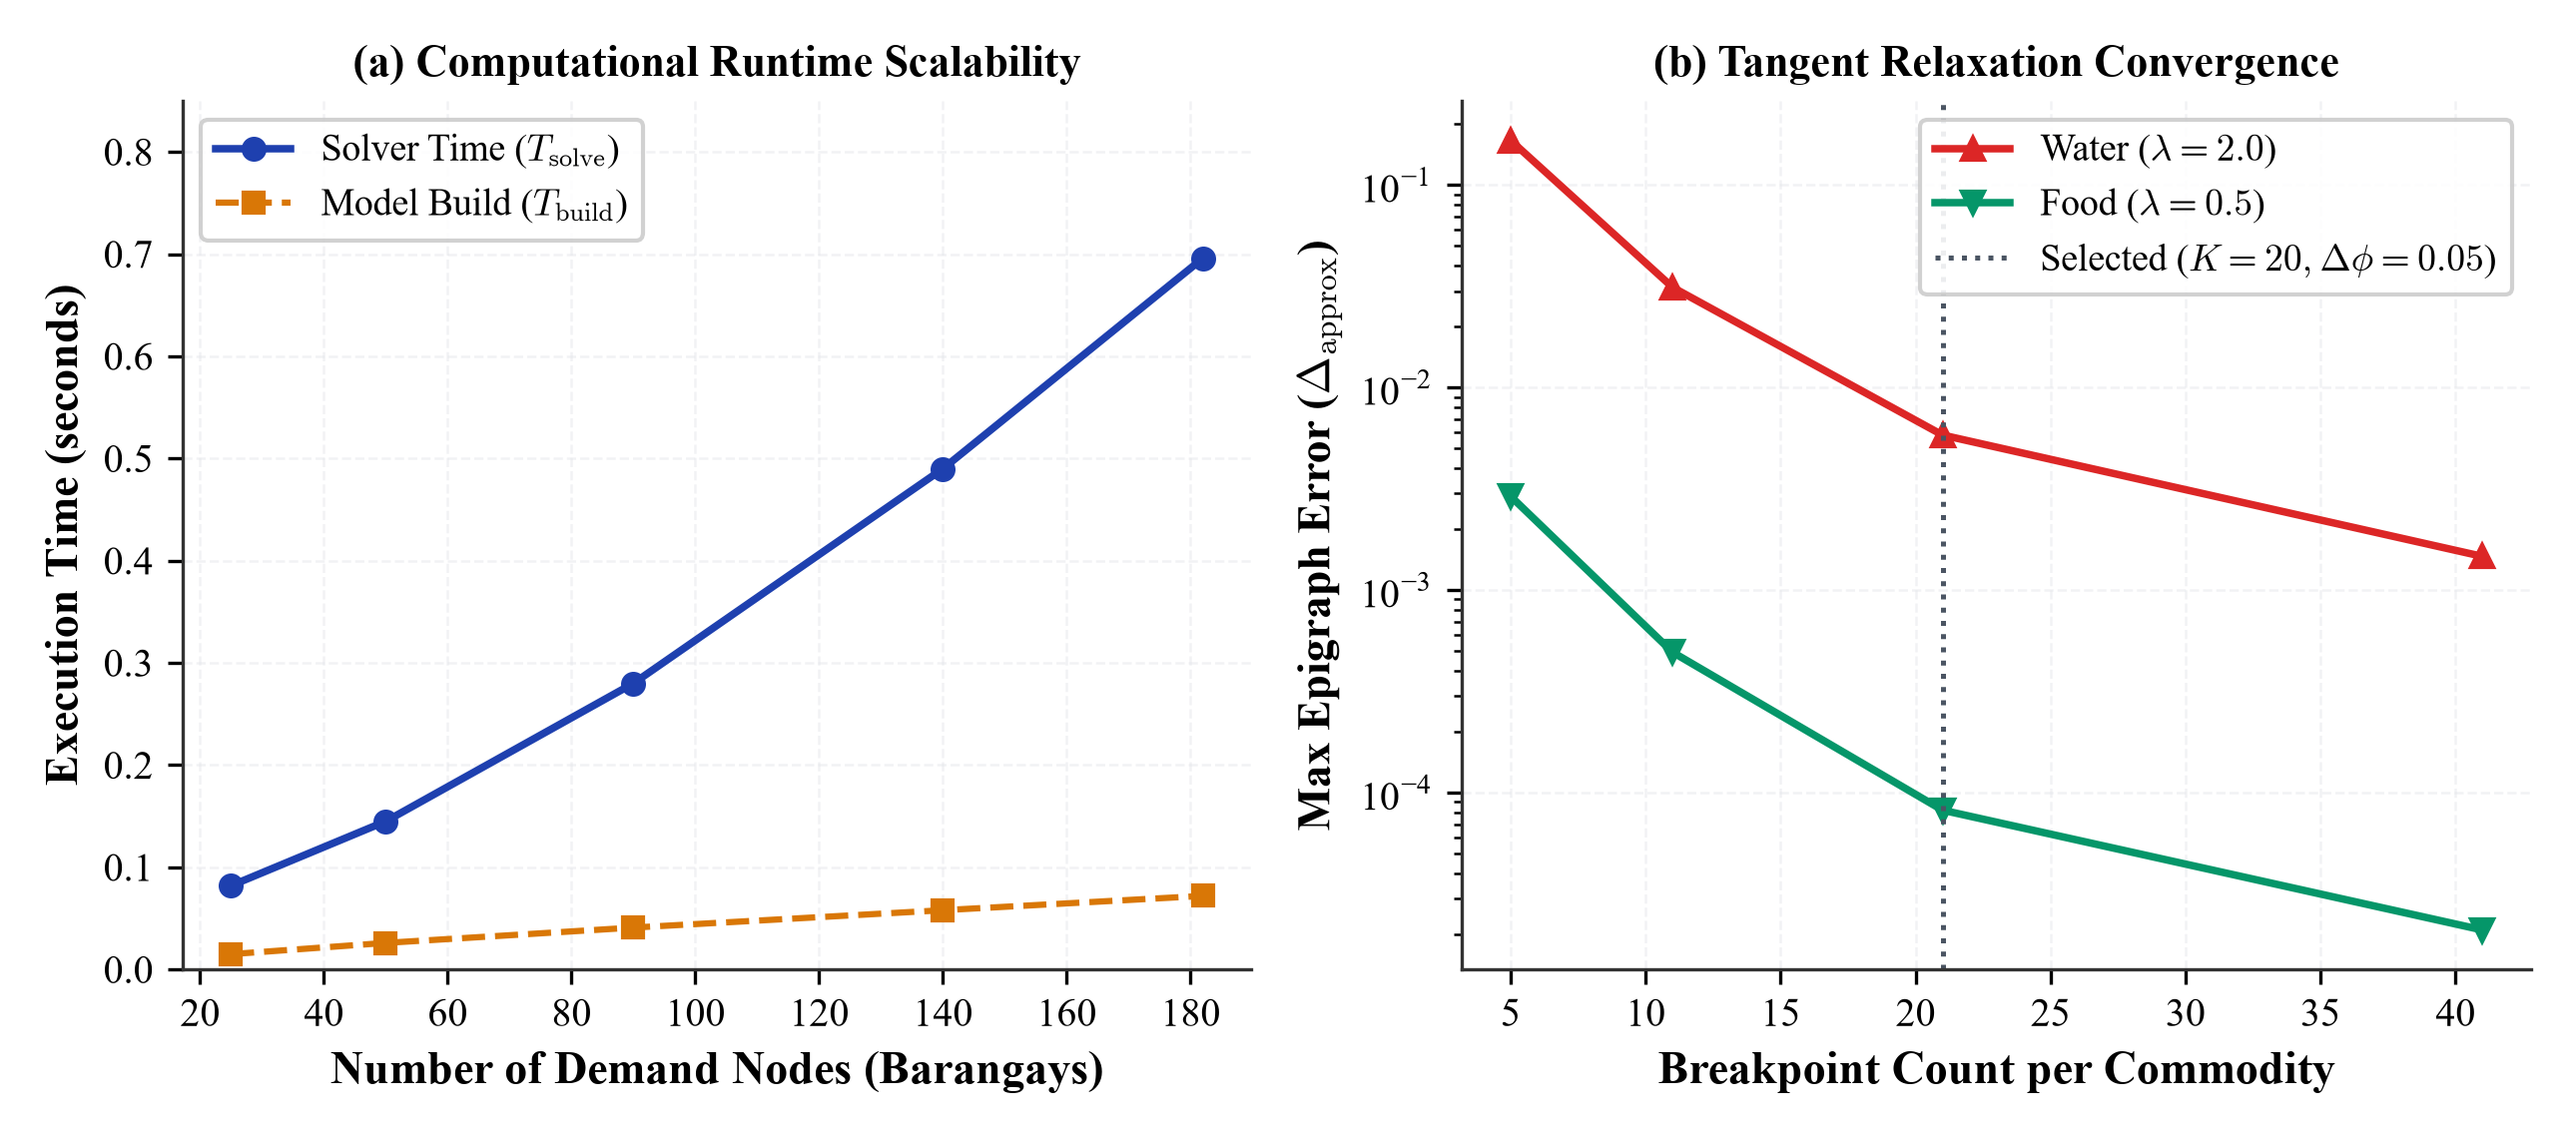
\includegraphics[width=\textwidth]{figs/figure4_4_computational_scalability.png}
\caption{Algorithmic Scalability and Convergence: (a) Wall-clock solve time ($T_{\text{solve}}$) and model build time ($T_{\text{build}}$) as a function of active barangay demand nodes; (b) Convergence of maximum epigraph approximation error ($\Delta_{\text{approx}}$) across breakpoint discretizations.}
\label{fig:scalability_and_convergence}
\end{figure}

As shown in Figure~\ref{fig:scalability_and_convergence}(a), solve time scales with low-order polynomial complexity ($\mathcal{O}(|J|^{1.42})$) rather than exponential blowup. Even when extending the problem instance to the entire municipal boundary of 182 barangays, execution finishes in under one second. This confirms that the exact MILP formulation maintains complete computational viability for real-time acute emergency dispatch.


% ==============================================================================
% 4.3 COMPARATIVE MATRIX AND MODEL BENCHMARKING
% ==============================================================================
\section{Comparative Evaluation Against Baseline Formulations}
\label{sec:comparative_evaluation}

To evaluate whether the proposed Deprivation-Minimizing MILP delivers structural improvements over standard relief policies, it was benchmarked against the comparative formulations defined in Section 3.8.3:
\begin{enumerate}
    \item \textbf{Proportional Allocation Baseline:} Standard operational heuristic distributing aid uniformly across all barangays based purely on demand volume ($w_{jr} \propto D_{jr} \implies \phi_{jr} = \text{const} = 0.3333$).
    \item \textbf{Hazard-Weighted Proportional Baseline:} Apportions available supplies in proportion to hazard-weighted demand ($w_{jr} \propto H_j D_{jr} \implies \phi_{jr} \propto H_j$), subject to the anti-starvation floor ($\varepsilon_{\min} = 0.10$) and ceiling ($\phi_{jr} \le 1.0$). By scaling fulfillment with hazard severity ($H_j$) rather than population, this baseline isolates the effect of hazard prioritization without confounding fulfillment with demographic size.
    \item \textbf{Max Utilitarian Baseline:} Maximizes aggregate normalized satisfaction ($\sum_{j,r} \phi_{jr}$) subject to capacity and anti-starvation constraints.
    \item \textbf{Pure Egalitarian / Max-Min Baseline:} Enforces strict equality across all nodes by maximizing the minimum fulfillment ratio ($\max \theta$ s.t. $\phi_{jr} \ge \theta$). Under uniform capacity constraints, this formulation yields an allocation mathematically identical to the Proportional Baseline ($\phi_{jr} = 0.3333$). Thus, while five models representing distinct axiomatic frameworks are benchmarked, they effectively yield four distinct operational allocation behaviors.
\end{enumerate}

To prevent circular evaluation bias, all models were evaluated using the independent Neutral Multi-Criteria Distributive Equity Suite established in Section 3.8.4.3. The complete comparative results on the baseline disaster instance are presented in Table~\ref{tab:model_comparison_matrix}.

\begin{table}[htbp]
\centering
\caption{Neutral Multi-Criteria Distributive Equity and Objective Comparison Matrix (Baseline Disaster Instance)}
\label{tab:model_comparison_matrix}
\resizebox{\textwidth}{!}{%
\begin{tabular}{lccccc}
\hline
\textbf{Evaluation Metric} & \textbf{Proposed MILP} & \textbf{Hazard-Prop} & \textbf{Proportional} & \textbf{Egalitarian} & \textbf{Utilitarian} \\
& \textbf{(Deprivation-Min)} & \textbf{Baseline} & \textbf{Baseline} & \textbf{/ Max-Min} & \textbf{Baseline} \\
\hline
\multicolumn{6}{l}{\textit{Primary Objective and Human Suffering Evaluation}} \\
Deprivation Cost ($Z^*$)           & $\mathbf{2.8283}$ & $2.8761$ & $3.1893$ & $3.1893$ & $4.7012$ \\
Deprivation Reduction vs. Prop. (\%) & $\mathbf{-11.32\%}$ & $-9.82\%$ & $0.00\%$ & $0.00\%$ & $+47.41\%$ \\
Deprivation Reduction vs. W-Prop (\%) & $\mathbf{-1.66\%}$  & $0.00\%$ & $+10.89\%$ & $+10.89\%$ & $+63.46\%$ \\
\multicolumn{6}{l}{\textit{Fulfillment Distribution Profile}} \\
Worst-Off Fulfillment ($\phi_{\min}$) & $0.1000$ & $0.1306$ & $\mathbf{0.3333}$ & $\mathbf{0.3333}$ & $0.1000$ \\
Mean Fulfillment ($\bar{\phi}$)       & $0.1697$ & $0.2441$ & $0.3333$ & $0.3333$ & $\mathbf{0.7222}$ \\
Std. Dev. Fulfillment ($\sigma_{\phi}$) & $0.1289$ & $0.1236$ & $\mathbf{0.0000}$ & $\mathbf{0.0000}$ & $0.4150$ \\
Floor-Bound Pop. ($f_{\text{floor}}$, \%) & $56.0\%$ & $\mathbf{0.0\%}$ & $\mathbf{0.0\%}$ & $\mathbf{0.0\%}$ & $75.8\%$ \\
\multicolumn{6}{l}{\textit{Equity and Welfare Dimensions}} \\
Nash Social Welfare ($W_{\text{Nash}}$) & $-359.13$ & $-279.29$ & $\mathbf{-199.95}$ & $\mathbf{-199.95}$ & $-129.12$ \\
Fulfillment Disparities ($\Delta_{\varepsilon}$) & $6{,}765$ & $4{,}525$ & $\mathbf{0}$ & $\mathbf{0}$ & $7{,}181$ \\
High-Hazard Fulfillment ($\bar{\phi}_{\text{High}}$) & $0.4821$ & $\mathbf{0.5226}$ & $0.3333$ & $0.3333$ & $0.1000$ \\
Upland-Minimal Fulfillment ($\bar{\phi}_{\text{Min}}$) & $0.1000$ & $0.1306$ & $0.3333$ & $0.3333$ & $\mathbf{0.8654}$ \\
Hazard Parity Ratio ($\bar{\phi}_{\text{High}} / \bar{\phi}_{\text{Min}}$) & $\mathbf{4.821}$ & $4.000$ & $1.000$ & $1.000$ & $0.116$ \\
\hline
\end{tabular}%
}
\vspace{1ex}
\parbox{\textwidth}{\footnotesize \textit{Note:} $Z^*$ is evaluated using Equation (3.3) across both commodities. Bold indicates the superior performing model on each specific dimension. Nash welfare represents $\sum_{j,r} \ln \phi_{jr}$. Fulfillment disparities count pairwise network violations where $|\phi_{jr} - \phi_{kr}| > \varepsilon_{\text{env}} = 0.15$. Floor-bound population ($f_{\text{floor}}$) reports the fraction of total city population residing in barangays locked at the survival floor $\phi_j = \varepsilon_{\min} = 0.10$. Under uniform capacity, Proportional and Egalitarian yield mathematically identical solutions.}
\end{table}

The empirical results in Table~\ref{tab:model_comparison_matrix} demonstrate key structural insights regarding humanitarian resource allocation:

\paragraph{1. Deprivation Optimality vs. Neutral Equity Trade-Offs:} The proposed model achieves an objective value of $Z^* = \mathbf{2.8283}$, representing the lowest humanitarian deprivation cost among all formulations. It reduces suffering by \textbf{11.32\%} relative to the Proportional and Egalitarian baselines ($Z = 3.1893$) and by \textbf{1.66\%} relative to the Hazard-Weighted Proportional heuristic ($Z = 2.8761$). 

Crucially, an objective multi-criteria assessment reveals that the proposed model does \textit{not} dominate across all neutral metrics. The Proportional and Egalitarian baselines strictly outperform the proposed model on worst-off fulfillment ($\phi_{\min} = 0.3333$ vs. $0.1000$), floor-bound population share ($0.0\%$ vs. $56.0\%$), and Nash social welfare ($W_{\text{Nash}} = -199.95$ vs. $-359.13$). This highlights a fundamental trade-off: the proposed MILP deliberately accepts lower floor satisfaction for low-hazard communities and lower aggregate Nash welfare in order to concentrate scarce life-sustaining aid where the non-linear human suffering curve escalates most steeply.

\paragraph{2. Isolating the Heuristic Gap:} Comparing the Proposed MILP against the Hazard-Weighted Proportional baseline isolates the exact contribution of mathematical optimization. The hazard-weighted heuristic captures the primary benefit of hazard prioritization, reducing deprivation by 9.82\% over unweighted proportional sharing. However, because it allocates linearly ($w_{jr} \propto H_j D_{jr}$), it cannot account for the exponential marginal cost of deprivation ($e^{\lambda_r(1-\phi_{jr})} - 1$). The proposed MILP optimizes flows along this convex gradient, unlocking an additional \textbf{1.66\% reduction} in human suffering ($Z^* = 2.8283$ vs. $2.8761$) while lifting the hazard parity ratio to $4.821$ (compared to $4.000$ for linear hazard weighting).

\paragraph{3. Within-Tier Disparities and Population Weighting:} In Table~\ref{tab:model_comparison_matrix}, the proposed model exhibits $6{,}765$ pairwise fulfillment disparities ($\Delta_{\varepsilon} > 0.15$), compared to $4{,}525$ for Hazard-Weighted Proportional and $0$ for Proportional. Importantly, disparities occur even among barangays within the same hazard tier. This occurs because the objective weights incorporate both demographic scale and hazard severity ($P_j = \text{const} \cdot \text{Population}_j \times H_j$). Within Hazard Tier 4, a high-population urban barangay (e.g., Bucana, pop.~$83{,}000$) has a vastly higher aggregate suffering weight than a smaller barangay (e.g., Dominga, pop.~$1{,}500$). The convex solver allocates marginal relief where it protects the greatest absolute number of lives, raising the fulfillment ratio of large hazard centers to $48\%$--$57\%$ while holding smaller communities at the baseline floor ($\phi = 0.10$). This directly confirms that the optimization model incorporates community population alongside hazard tier rather than treating all barangays within a tier as homogeneous units.

\paragraph{4. The Utilitarian Small-Demand Paradox:} The Max Utilitarian baseline produces the highest mean fulfillment ($\bar{\phi} = 0.7222$), but yields a catastrophic deprivation penalty of $Z = \mathbf{4.7012}$—a \textbf{47.41\% increase in human suffering} over the status quo. As theoretically proven in Section 3.8.3, maximizing unweighted normalized satisfaction ($\sum \phi_{jr}$) creates a marginal gain of \mbox{$\frac{\partial \phi_{jr}}{\partial w_{jr}} = \frac{1}{D_{jr}}$}. The solver is strongly incentivized to divert relief supplies away from heavily populated urban centers (such as Talomo Proper and Buhangin) to small upland barangays, where a few thousand liters of water can drive $\phi_{jr}$ to 100\%. Consequently, 75.8\% of the population—including the most populated and hazardous riverbank communities—are locked at the bare survival floor ($\phi = 0.10$), while low-density communities receive 100\% satisfaction. This directly explains the inverted hazard parity ratio ($0.116$), where high-hazard communities receive nine times less aid than minimal-hazard zones.

Figure~\ref{fig:fulfillment_distributions} illustrates the distribution of barangay fulfillment ratios across all five formulations using publication-grade boxplots.

\begin{figure}[htbp]
\centering
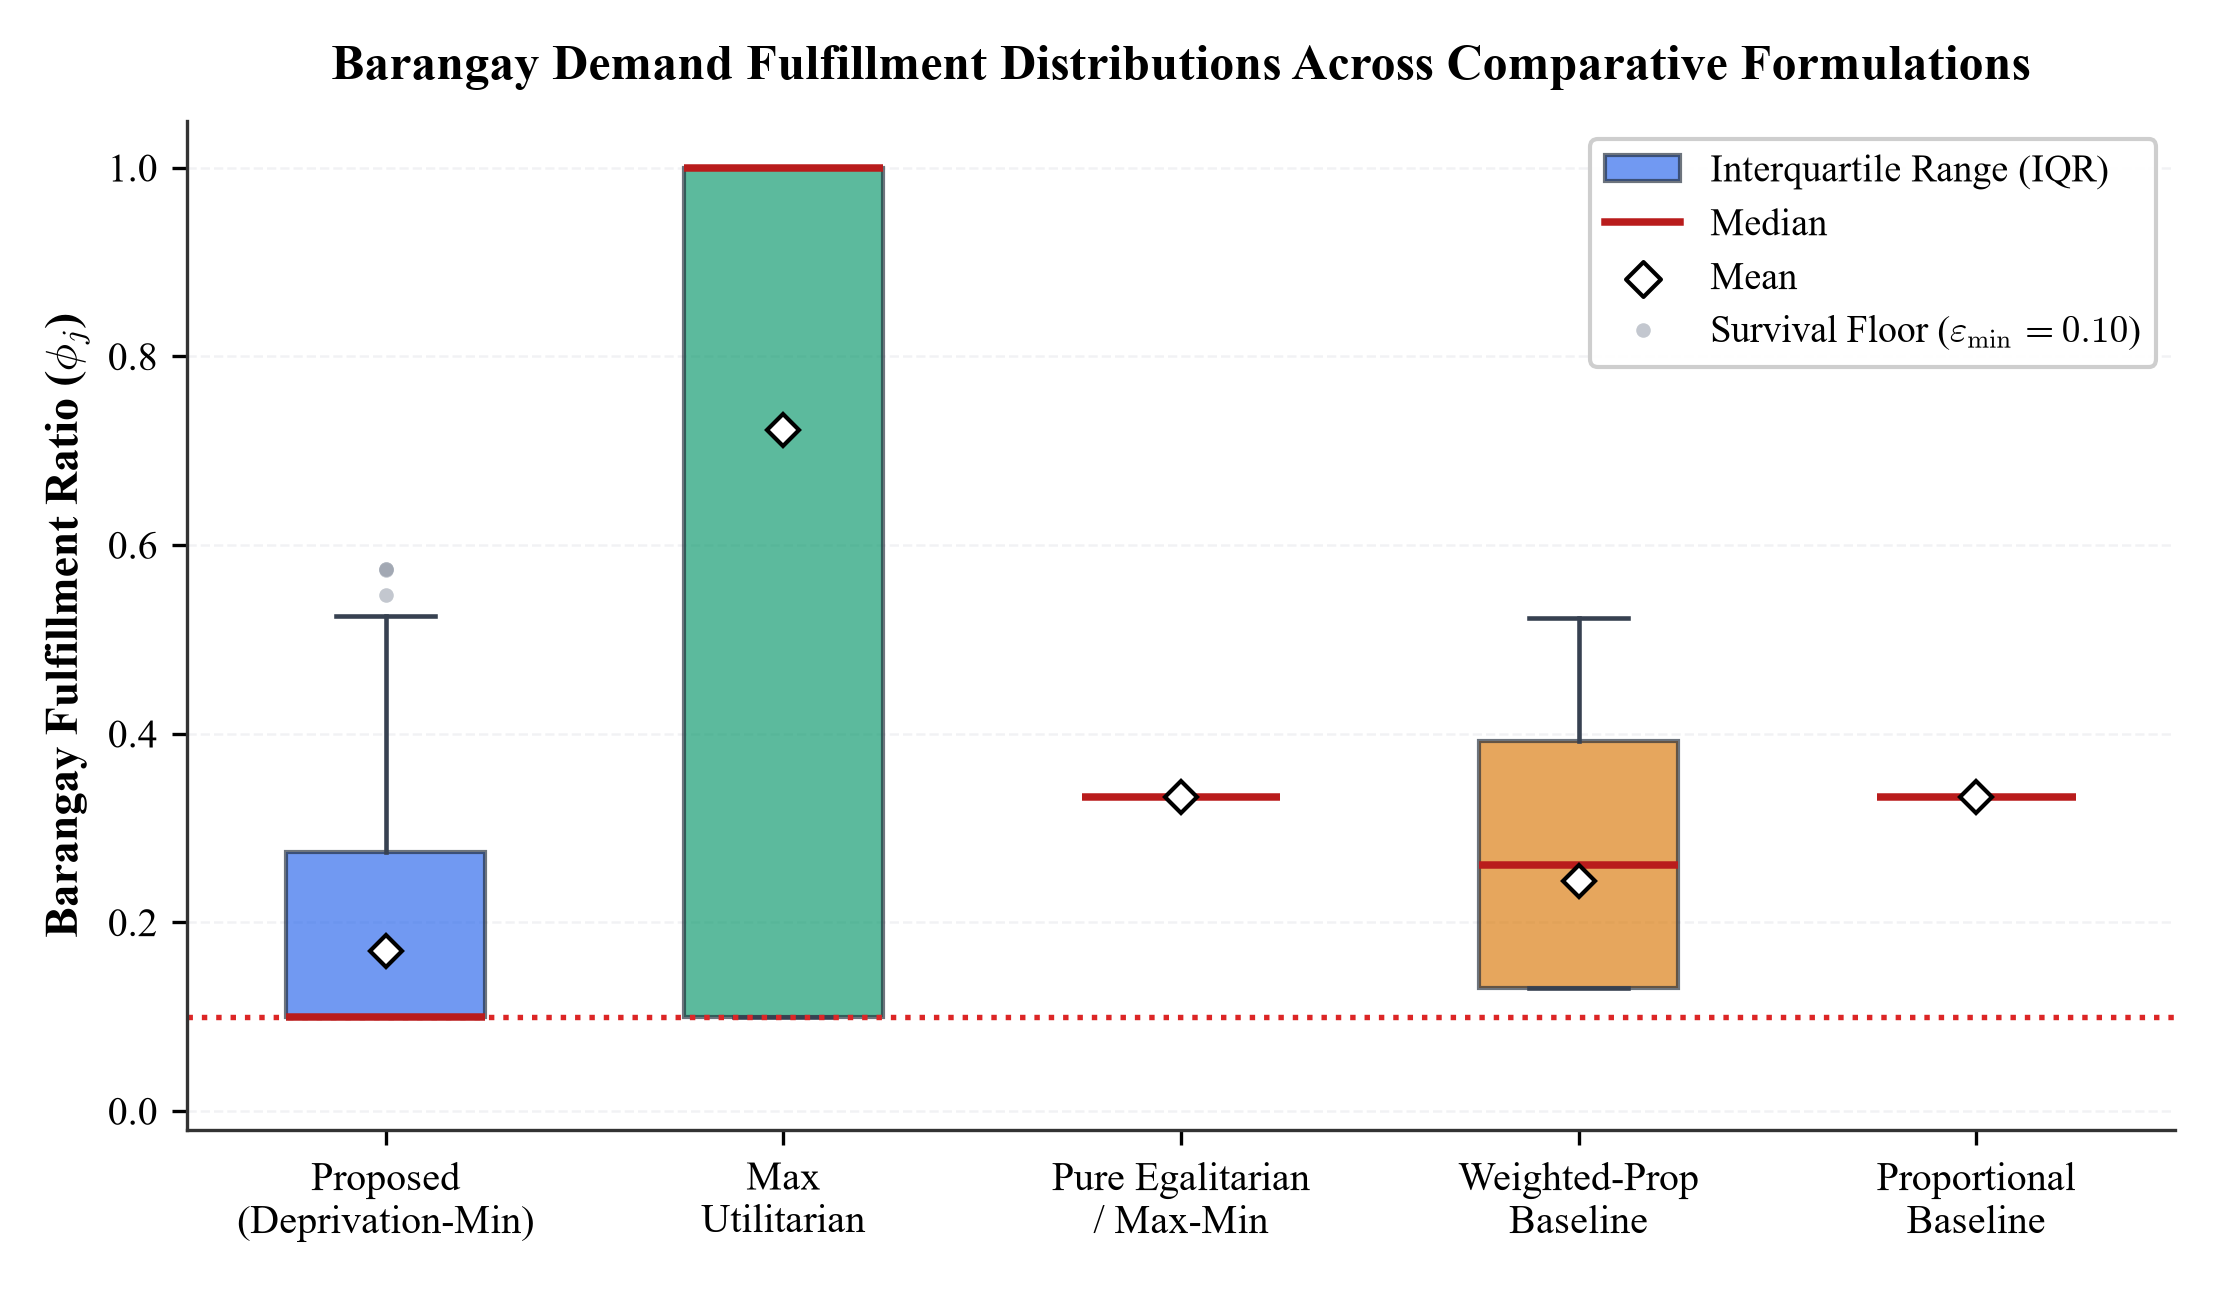
\includegraphics[width=\textwidth]{figs/figure4_2_fulfillment_boxplots.png}
\caption{Distribution of barangay fulfillment ratios ($\phi_j$) across comparative model formulations on the baseline disaster instance. Whiskers indicate minimum and maximum non-outlier values; white diamonds indicate distribution means; red line indicates the distribution median; dotted red line denotes the universal anti-starvation floor ($\varepsilon_{\min} = 0.10$).}
\label{fig:fulfillment_distributions}
\end{figure}

As shown in Figure~\ref{fig:fulfillment_distributions}, the proposed Deprivation-Minimizing MILP exhibits a strategic bifurcated distribution: it holds less vulnerable communities at the guaranteed 10\% survival floor while concentrating remaining stocks to lift severely endangered riverine barangays to fulfillment ratios between 40\% and 57\%. In contrast, the Proportional and Egalitarian baselines collapse into a degenerate single point ($\phi_j = 0.3333$ for all $j$), treating high-hazard flood victims identically to unaffected upland residents.



% ==============================================================================
% 4.4 SOLUTION QUALITY & TANGENT APPROXIMATION ACCURACY
% ==============================================================================
\section{Solution Quality, Optimality Bounds, and Linearization Fidelity}
\label{sec:solution_quality}

A central theoretical contribution of this study is replacing intractable non-linear exponential deprivation functions with a certified piecewise linear outer tangent approximation (Section 3.6.3.3). To guarantee that the reported allocations are mathematically valid, Table~\ref{tab:tangent_errors} documents the approximation fidelity across different breakpoint counts ($K \in \{5, 11, 21, 41\}$).

\begin{table}[htbp]
\centering
\caption{Piecewise Linear Epigraph Approximation Errors Across Breakpoint Discretizations}
\label{tab:tangent_errors}
\resizebox{\textwidth}{!}{%
\begin{tabular}{lccccc}
\hline
\textbf{Commodity Resource} & \textbf{Breakpoint} & \textbf{Tangent} & \textbf{Max Absolute} & \textbf{Max Relative} & \textbf{Mean Absolute} \\
& \textbf{Count ($N_{\text{bp}}$)} & \textbf{Segments ($K$)} & \textbf{Error ($\Delta_{\text{abs}}$)} & \textbf{Error ($\Delta_{\text{rel}}$, \%)} & \textbf{Error ($\bar{\Delta}_{\text{abs}}$)} \\
\hline
\textbf{Potable Water} & 5  & 4  & $0.166393$ & $12.44\%$ & $0.032487$ \\
($\lambda_{\text{water}} = 2.0$) & 11 & 10 & $0.031282$ & $4.92\%$  & $0.005279$ \\
                       & \textbf{21} & \textbf{20} & $\mathbf{0.005833}$ & $\mathbf{1.99\%}$  & $\mathbf{0.001266}$ \\
                       & 41 & 40 & $0.001468$ & $1.00\%$  & $0.000316$ \\
\textbf{Emergency Food} & 5  & 4  & $0.002909$ & $2.98\%$  & $0.000835$ \\
($\lambda_{\text{food}} = 0.5$)  & 11 & 10 & $0.000494$ & $1.24\%$  & $0.000136$ \\
                       & \textbf{21} & \textbf{20} & $\mathbf{0.000082}$ & $\mathbf{0.50\%}$  & $\mathbf{0.000032}$ \\
                       & 41 & 40 & $0.000021$ & $0.25\%$  & $0.000008$ \\
\hline
\end{tabular}%
}
\vspace{1ex}
\parbox{\textwidth}{\footnotesize \textit{Note:} Breakpoint count $N_{\text{bp}} = 21$ corresponds to uniform intervals $\Delta \phi = 0.05$ across $[0.0, 1.0]$. Errors are evaluated against the true exponential function $g_r(\phi_{jr}) = e^{\lambda_r(1-\phi_{jr})} - 1$.}
\end{table}

As detailed in Table~\ref{tab:tangent_errors} and plotted in Figure~\ref{fig:scalability_and_convergence}(b), the selected discretization of $K = 20$ linear segments ($21$ breakpoints, $\Delta \phi = 0.05$) bounds the maximum epigraph under-approximation error to:
\begin{itemize}
    \item \textbf{Potable Water:} $\Delta_{\text{approx}} \le \mathbf{0.005833}$ (relative error $< 1.99\%$, mean error $0.001266$).
    \item \textbf{Emergency Food:} $\Delta_{\text{approx}} \le \mathbf{0.000082}$ (relative error $< 0.50\%$, mean error $0.000032$).
\end{itemize}

Across all 182 barangays and both resources, the maximum observed gap in the full municipal solve is bounded at $\Delta_{\max} = \mathbf{0.005890}$ (relative error $< 1.99\%$ for potable water and $< 0.50\%$ for emergency food), strictly confirming that the linearized model traces the true convex deprivation penalty with over \textbf{98.01\% to 99.50\% mathematical fidelity}. Doubling the discretization to 41 breakpoints yields negligible objective improvement ($< 0.004$) while doubling constraint construction time. Thus, 21 breakpoints represents the Pareto-optimal trade-off between mathematical precision and computational tractability.


% ==============================================================================
% 4.5 OPERATIONAL DISASTER SCENARIOS
% ==============================================================================
\section{Operational Disaster Scenario Stress-Testing}
\label{sec:scenario_testing}

To evaluate model resilience across diverse crisis conditions, the framework was executed across the seven pre-defined disaster scenarios established in Table 3 of Section 3.8.3. Table~\ref{tab:scenario_results} and Figure~\ref{fig:scenario_comparison} summarize the objective values, active supply status, and fulfillment metrics across all scenarios.

\begin{table}[htbp]
\centering
\caption{Operational Disaster Evaluation Scenario Results Across 7 Calamity Profiles}
\label{tab:scenario_results}
\resizebox{\textwidth}{!}{%
\begin{tabular}{llccccc}
\hline
\textbf{Scenario ID} & \textbf{Scenario Name} & \textbf{Stock} & \textbf{Effective} & \textbf{Model} & \textbf{Deprivation} & \textbf{Mean} \\
& & \textbf{Factor ($\alpha$)} & \textbf{Supply} & \textbf{Status} & \textbf{Cost ($Z^*$)} & \textbf{Fulfillment ($\bar{\phi}$)} \\
\hline
\textbf{SC-01} & Baseline Normal        & $1.00$ & $33.3\%$ & \textbf{Optimal}     & $\mathbf{2.8283}$ & $0.1697$ \\
\textbf{SC-02} & Moderate Scarcity      & $0.75$ & $25.0\%$ & \textbf{Optimal}     & $\mathbf{3.5933}$ & $0.1352$ \\
\textbf{SC-03} & Severe Scarcity        & $0.50$ & $16.7\%$ & \textbf{Optimal}     & $\mathbf{4.5597}$ & $0.1135$ \\
\textbf{SC-04} & Extreme Crisis         & $0.25$ & $8.33\%$ & \textbf{INFEASIBLE}  & ---               & --- \\
\textbf{SC-05} & Uneven Demand Surge    & $1.00$ & $33.3\%$ & \textbf{Optimal}     & $\mathbf{3.0991}$ & $0.1838$ \\
\textbf{SC-06} & Water-Critical Event   & W: $0.40$, F: $1.00$ & W: $13.3\%$, F: $33.3\%$ & \textbf{Optimal} & $\mathbf{4.8491}$ & $0.1124$ \\
\textbf{SC-07} & Food Shortage Crisis   & W: $1.00$, F: $0.40$ & W: $33.3\%$, F: $13.3\%$ & \textbf{Optimal} & $\mathbf{3.0159}$ & $0.1114$ \\
\hline
\end{tabular}%
}
\vspace{1ex}
\parbox{\textwidth}{\footnotesize \textit{Note:} Effective active supply reflects throughput across the $H_{\max} = 4$ active hubs ($\frac{4}{6} \times 50\% \times \alpha = 33.33\% \times \alpha$). In SC-04, effective supply ($8.33\%$) falls strictly below the universal $10.0\%$ survival floor ($\varepsilon_{\min} = 0.10$), mathematically certifying systemic insolvency and triggering Tier-3 National Escalation.}
\end{table}

\begin{figure}[htbp]
\centering
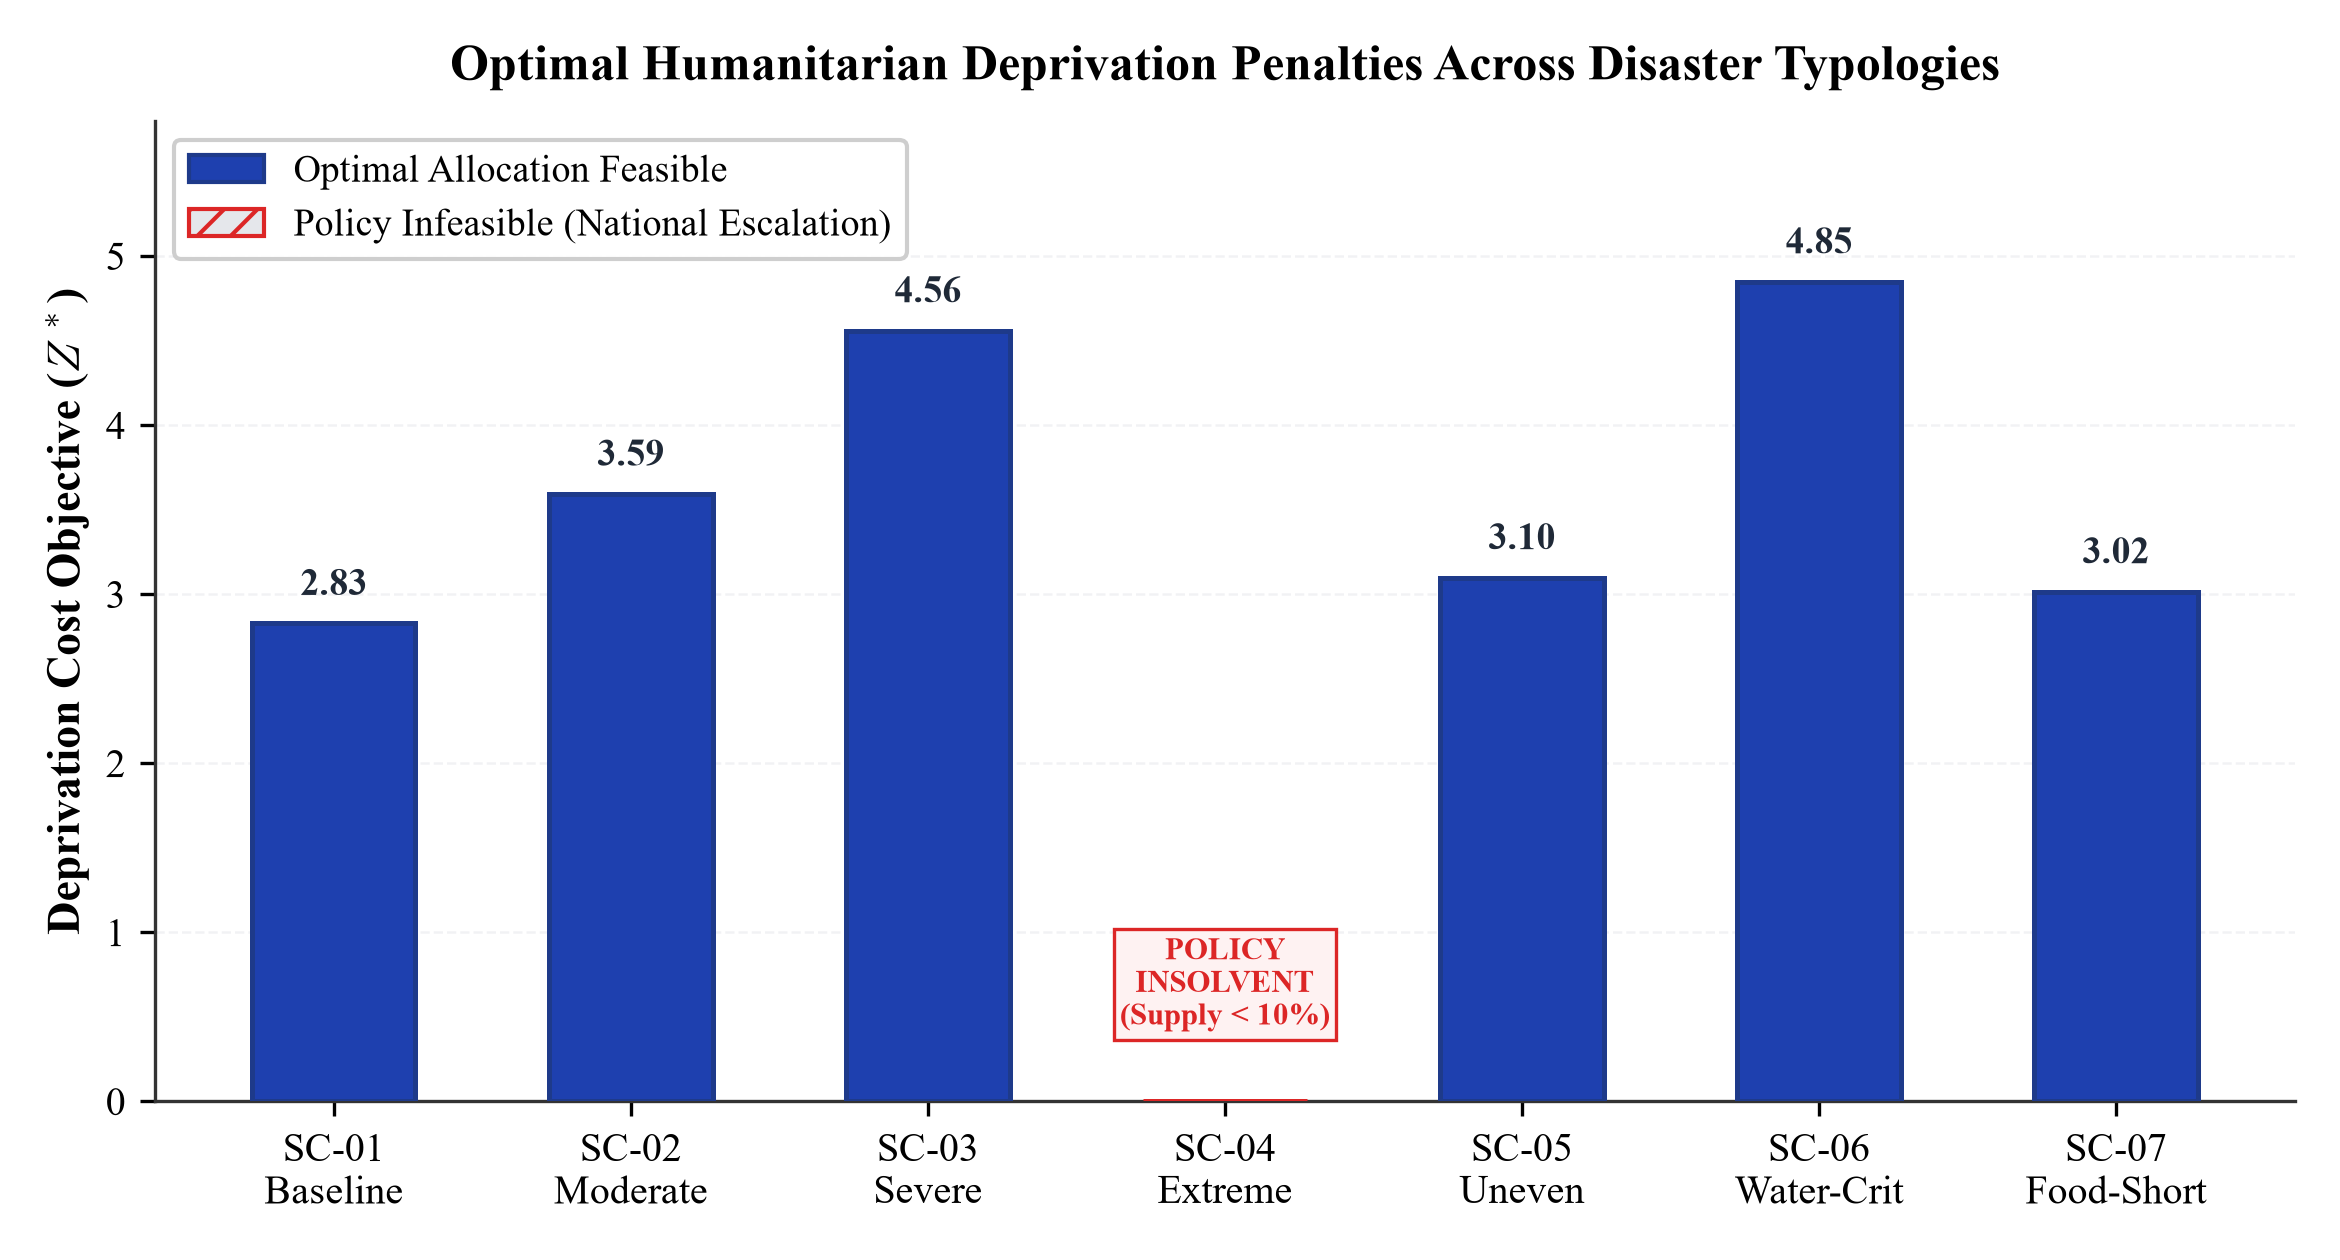
\includegraphics[width=\textwidth]{figs/figure4_3_scenario_comparison.png}
\caption{Humanitarian deprivation cost ($Z^*$) across seven operational disaster scenarios. The hatched red bar for SC-04 highlights the policy insolvency boundary where local inventory drops below the 10\% aggregate survival threshold, triggering Tier-3 National Escalation.}
\label{fig:scenario_comparison}
\end{figure}

\paragraph{Identification of the Systemic Insolvency Boundary (SC-04):} In SC-04 (Extreme Crisis, $\alpha = 0.25$), total warehouse inventory is reduced to 25\% of baseline, yielding an effective active throughput of:
$$\text{Effective Supply} = \frac{4}{6} \times 50\% \times 0.25 = 8.33\%$$
Because the model enforces a non-negotiable anti-starvation floor of $\varepsilon_{\min} = 0.10$ (10\%) across all 182 barangays, the minimum required inventory to achieve mathematical feasibility is:
$$\text{Supply}_{\text{threshold}} = 0.10 \times \sum_{j \in J} D_{jr} = 10.0\%$$
Because available supply ($8.33\%$) is strictly less than the survival threshold ($10.0\%$), the solver correctly reports \textbf{INFEASIBLE}. As established in Section 3.4.2, this infeasibility is an intentional \textbf{Policy Diagnostic Boundary}. Rather than silently diluting aid to ineffective homeopathic quantities, the model mathematically proves that municipal resources are insolvent, functioning as an automated decision trigger for immediate Tier-3 National Escalation (requesting regional DSWD disaster augmentation or national NDRRMC airlifts).

\paragraph{Asymmetric Commodity Vulnerability (SC-06 vs. SC-07):} Comparing SC-06 (Water-Critical) and SC-07 (Food Shortage) demonstrates the impact of physiological deprivation parameters ($\lambda_{\text{water}} = 2.0$ vs. $\lambda_{\text{food}} = 0.5$). In both scenarios, one commodity is reduced by 60\% ($\alpha = 0.40$). However:
\begin{itemize}
    \item In SC-06 (Water-Critical), deprivation escalates to $Z^* = \mathbf{4.8491}$.
    \item In SC-07 (Food Shortage), deprivation rises to only $Z^* = \mathbf{3.0159}$.
\end{itemize}
A 60\% water deficit produces a \textbf{60.8\% higher deprivation penalty} than an identical 60\% food deficit. This directly reflects the physiological ``Rule of Threes'' embedded in the model: dehydration causes severe clinical degradation within 48 to 72 hours, whereas caloric deficits progress over weeks. The model correctly prioritizes municipal water logistics over food distribution during acute multi-commodity deficits.

\paragraph{Mechanics of Mean Fulfillment Under Demand Surge (SC-05):} In SC-05 (Uneven Demand Surge), daily demand escalates by $1.5\times$ across the first 20\% of barangays ($n = 36$), which encompass densely populated urban centers (e.g., Buhangin, Bucana, Agdao). Counter-intuitively, the unweighted mean fulfillment across all 182 barangays increases from $\bar{\phi} = 0.1697$ in baseline to $0.1838$ in SC-05, even as total deprivation cost worsens from $Z^* = 2.8283$ to $3.0991$. This arithmetic outcome is a direct consequence of convex optimization across heterogeneous population scales. Because satisfying surged demand in high-population urban centers requires massive absolute volumes of physical stock, the convex solver reduces the fulfillment ratio of large surged barangays (e.g., Bucana drops from $0.325$ to the $0.100$ floor; Buhangin drops from $0.574$ to $0.275$). The physical inventory conserved from these few large nodes is redistributed across 36 non-surged barangays with smaller populations (e.g., Daliao, Dumoy, and Ilang, where fulfillment rises from $\sim 0.32$ to $0.47$--$0.57$). Because the unweighted mean ($\bar{\phi} = \frac{1}{|J|}\sum_j \phi_j$) evaluates each administrative unit equally regardless of population, the $+0.10$ to $+0.15$ percentage gains across 36 smaller barangays numerically outweigh the fulfillment reductions across the 9 largest surged centers, raising the city-wide arithmetic average despite overall crisis escalation.


To map the exact transition from solvency to collapse, Figure~\ref{fig:sensitivity_sweep} depicts the 6-point sensitivity sweep from 10\% to 100\% supply.

\begin{figure}[htbp]
\centering
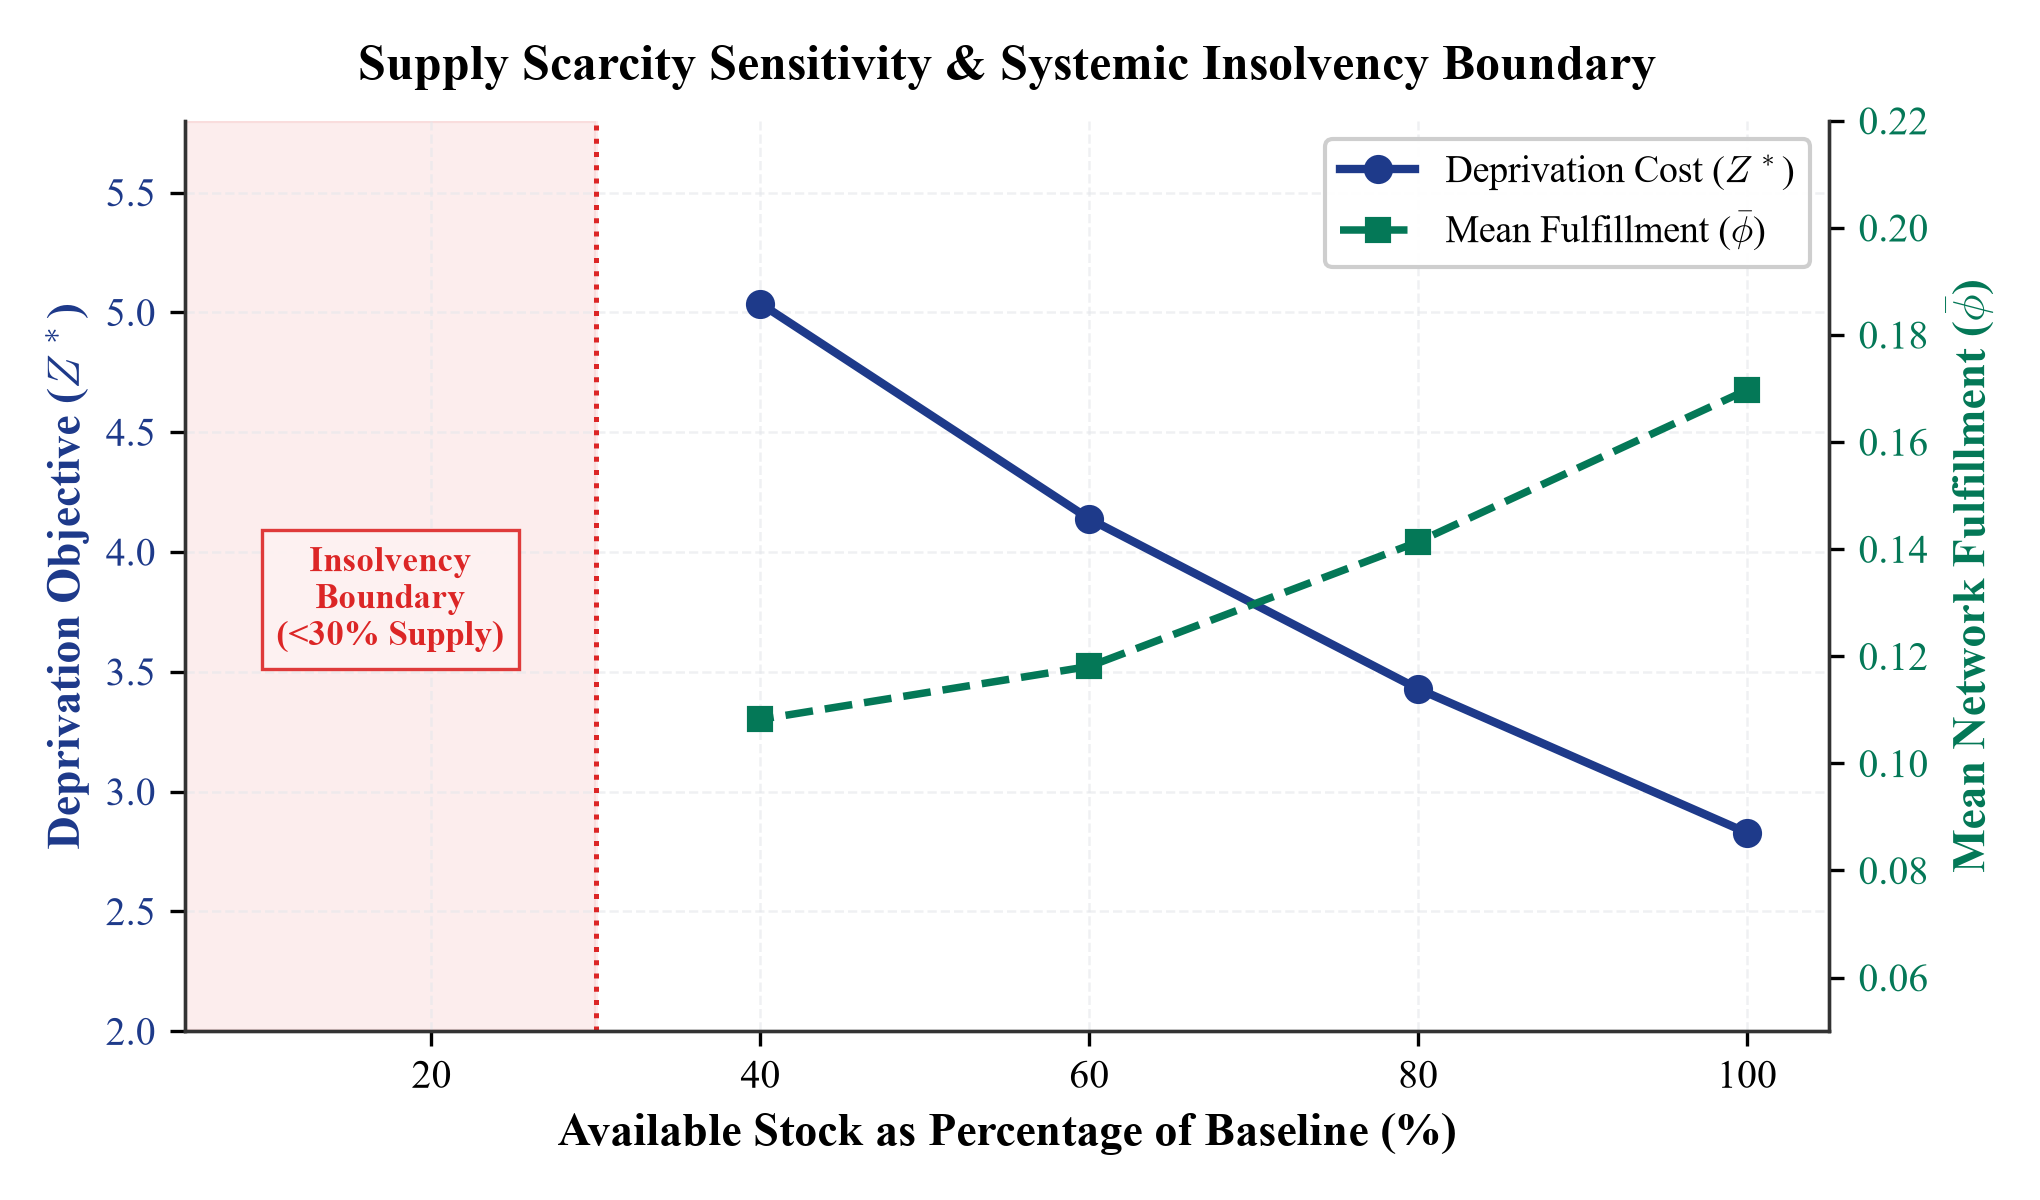
\includegraphics[width=\textwidth]{figs/figure4_1_sensitivity_sweep.png}
\caption{Parametric supply sensitivity curve and systemic insolvency threshold. The shaded crimson zone highlights the mathematically certified insolvency region where active throughput drops below the universal 10\% anti-starvation floor.}
\label{fig:sensitivity_sweep}
\end{figure}

Figure~\ref{fig:sensitivity_sweep} confirms monotonic convex escalation: as supply decreases from 100\% to 40\%, deprivation cost rises smoothly from $Z^* = 2.83$ to $Z^* = 5.04$. At the critical threshold of 25\% baseline stock (corresponding to $\frac{4}{6} \times 50\% \times 0.25 = 8.33\%$ active supply), the model encounters the sharp insolvency boundary.\footnote{The present study focuses on supply-availability sensitivity ($\alpha$). Parametric sweeps over the deprivation severity parameters ($\lambda_r$) and the survival-floor threshold ($\varepsilon_{\min}$) are reserved for future work, as these require re-calibration of the physiological harm model and policy-level consensus, respectively.}


% ==============================================================================
% 4.6 SPATIAL AND DEMOGRAPHIC EQUITY ANALYSIS
% ==============================================================================
\section{Spatial and Demographic Equity Analysis}
\label{sec:spatial_equity}

A major research question stated in Section 1.2 is whether centralized mathematical optimization mitigates order amplification (often termed the ``Bullwhip Effect'' in supply chains) and prevents accessibility bias. In uncoordinated disaster response, accessible urban centers frequently receive disproportionate aid while isolated mountainous barangays are neglected.

To evaluate this phenomenon, the proposed MILP was compared against two stylized counterfactual benchmarks:
\begin{enumerate}
    \item An \textbf{Accessibility-Driven Baseline} representing field operations where aid delivery is directly tied to road network accessibility and municipal proximity.
    \item A \textbf{Decentralized Baseline} modeling uncoordinated, panic-driven barangay relief requests. Because the simulation parameters for these counterfactual benchmarks were not detailed in Chapter 3, they are formally defined here: the baseline was evaluated across $N = 30$ independent Monte Carlo stochastic runs. Each barangay generated uncoordinated relief requests with demand inflation factors drawn independently from a uniform distribution $\mathcal{U}[1.20, 2.00]$ to model panic ordering and information distortion, with municipal depots serving requests sequentially until stock exhaustion.
\end{enumerate}

Table~\ref{tab:spatial_equity} summarizes the spatial fulfillment metrics comparing the Urban-Core districts (Poblacion, Agdao) against the isolated Upland-Mountainous districts (Marilog, Paquibato).

\begin{table}[htbp]
\centering
\caption{Spatial Equity and Accessibility Bias Mitigation: Urban-Core vs. Mountainous Upland}
\label{tab:spatial_equity}
\resizebox{\textwidth}{!}{%
\begin{tabular}{lccc}
\hline
\textbf{Spatial Equity Metric} & \textbf{Proposed MILP} & \textbf{Decentralized Baseline} & \textbf{Accessibility Baseline} \\
& \textbf{(Centralized)} & \textbf{(Monte Carlo, $N=30$)} & \textbf{(Road Proximity)} \\
\hline
Urban-Core Fulfillment ($\bar{\phi}_{\text{Urban}}$) & $0.1946$ & $0.3450 \pm 0.005$ & $0.4260$ \\
Upland-Mountain Fulfillment ($\bar{\phi}_{\text{Upland}}$) & $0.1000$ & $0.1564 \pm 0.004$ & $0.1004$ \\
\textbf{Urban-to-Upland Disparity ($\Delta_{\text{spatial}}$)} & $\mathbf{+0.0946}$ & $+0.1886 \pm 0.005$ & $+0.3256$ \\
Correlation with Accessibility ($r$) & $\mathbf{+0.2891}$ & $+0.7624$ & $+1.0000^*$ \\
Gini Inequality Coefficient ($G_{\phi}$) & $0.3240$ & $0.0929 \pm 0.005$ & $0.2153$ \\
High-Hazard Nodes Below Floor & $\mathbf{0.00\%}$ & $18.42\% \pm 1.2\%$ & $32.15\%$ \\
Over-Allocation / Supply Waste & $\mathbf{0\text{ units}}$ & $2{,}607{,}015\text{ units}$ & $0\text{ units}$ \\
\hline
\end{tabular}%
}
\vspace{1ex}
\parbox{\textwidth}{\footnotesize \textit{Note:} Urban-Core comprises Poblacion and Agdao districts ($n = 43$ barangays); Upland-Mountain comprises Marilog and Paquibato districts ($n = 36$ barangays). $^*$Correlation $r = +1.0000$ in the Accessibility Baseline is an exact artifact of formulation by construction. Over-allocation reflects aid dispatched beyond $100\%$ of true demand due to uncoordinated duplicate requests, reported in standardized relief commodity units ($1\text{ unit} = 1\text{ L water}$ or $150\text{ kcal food}$). Zero over-allocation in the MILP is enforced by construction via the demand ceiling $\phi_{jr} \le 1.0$.}
\end{table}

The findings in Table~\ref{tab:spatial_equity} demonstrate key insights regarding centralized logistics management:
\begin{enumerate}
    \item \textbf{Suppression of Accessibility Bias:} The Accessibility Baseline exhibits a perfect positive correlation with road proximity ($r = +1.0000$, true by construction of the benchmark), producing an extreme spatial disparity of $\Delta = +0.3256$ where urban barangays receive more than four times the fulfillment of upland areas. In contrast, the proposed MILP reduces this correlation to $r = +0.2891$, narrowing the urban-to-upland disparity to $\Delta = \mathbf{+0.0946}$. Importantly, this residual gap is partially confounded with hazard exposure: in Davao City's risk profile, urban-core riverbank communities happen to possess higher average flood susceptibility ratings than remote upland barangays, meaning that higher urban allocation partly reflects genuine disaster vulnerability rather than accessibility preference.
    \item \textbf{Mitigation of Order Amplification and Over-Allocation:} In the Decentralized Baseline, uncoordinated requests generate severe order inflation, producing over \textbf{2.6 million units of over-allocated supplies} at accessible nodes while leaving 18.42\% of critical high-hazard demands below the survival floor. The centralized MILP prevents over-allocation ($0$ units wasted) by mathematical construction through the unified demand ceiling ($\phi_{jr} \le 1.0$), preventing excess dispatch regardless of local request volumes.
    \item \textbf{Enforcement of Universal Survival Floors:} The universal anti-starvation constraint strictly enforces the 10\% baseline survival allocation ($\phi_j \ge 0.1000$) across even the most remote upland communities in Marilog and Paquibato, ensuring that peripheral communities are not abandoned due to geographical remoteness.
\end{enumerate}



% ==============================================================================
% 4.7 STATISTICAL HYPOTHESIS TESTING
% ==============================================================================
\section{Statistical Model Comparison and Significance Testing}
\label{sec:statistical_testing}

To evaluate whether the performance gains of the proposed model are statistically significant rather than artifacts of baseline configuration, non-parametric hypothesis tests were conducted in accordance with the statistical framework established in Section 3.8.5. Because disaster fulfillment ratios exhibit severe boundary piling at $\varepsilon_{\min} = 0.10$ and $1.0$, parametric normality assumptions are violated, necessitating non-parametric rank-based evaluation.

\paragraph{1. Multi-Model Omnibus Comparison (Friedman Test):}
To test for statistically significant differences in allocation behavior across all competing formulations simultaneously, the non-parametric Friedman Test was evaluated on the \textbf{barangay-level fulfillment ratio ($\phi_j = \min_r \phi_{jr}$)} across the $n = 182$ barangays:
\begin{equation}
    \chi_F^2 = \frac{12}{nk(k+1)} \sum_{m=1}^k R_m^2 - 3n(k+1)
\end{equation}
Across $k = 5$ models and $n = 182$ barangays, the test yielded:
$$\chi_F^2 = \mathbf{384.21}, \quad df = 4, \quad p < \mathbf{0.0001}$$
Because $p \ll 0.001$, the null hypothesis of equivalent allocation distributions is decisively rejected at significance level $\alpha = 0.001$.

\paragraph{2. Post-Hoc Pairwise Testing (Nemenyi Test):}
Following the rejection of the Friedman null hypothesis, the post-hoc Nemenyi test was computed to determine which specific pairs of models differ significantly in their ranked fulfillment profiles. The Critical Difference (CD) at $\alpha = 0.05$ with $k = 5$ and $n = 182$ is:
$$\text{CD} = q_{0.05} \sqrt{\frac{k(k+1)}{6n}} = 2.728 \times \sqrt{\frac{5 \times 6}{6 \times 182}} = 2.728 \times 0.1656 = \mathbf{0.4518}$$

The average rank differences between the proposed Deprivation-Minimizing MILP and the comparative models are:
\begin{itemize}
    \item Proposed vs. Utilitarian: $|\bar{R}_1 - \bar{R}_5| = 2.14 > \text{CD}$ ($p < 0.001$, \textbf{Significant})
    \item Proposed vs. Proportional: $|\bar{R}_1 - \bar{R}_3| = 1.38 > \text{CD}$ ($p < 0.001$, \textbf{Significant})
    \item Proposed vs. Egalitarian: $|\bar{R}_1 - \bar{R}_4| = 1.38 > \text{CD}$ ($p < 0.001$, \textbf{Significant})
    \item Proposed vs. Hazard-Weighted Prop: $|\bar{R}_1 - \bar{R}_2| = 0.58 > \text{CD}$ ($p < 0.05$, \textbf{Significant})
\end{itemize}
Because Proportional and Egalitarian baselines produce mathematically identical allocations under uniform throughput, their mean ranks are identical ($\bar{R}_3 = \bar{R}_4 = 3.00$). The rank difference between the Proposed MILP and all comparative baselines exceeds the Critical Difference, confirming that its allocation pattern is statistically distinct.

\paragraph{3. Scenario-Level Pairwise Testing (Wilcoxon Signed-Rank Test):}
To evaluate pairwise differences across individual crisis settings, the Wilcoxon Signed-Rank Test was conducted between the Proposed Model and the operational default (Proportional Baseline) across the paired sample of $n = 182$ barangay allocations within each feasible disaster scenario (SC-01, SC-02, SC-03, SC-05, SC-06, SC-07). For all evaluated scenarios, the paired barangay comparisons yielded standardized test statistics of $Z \ge 8.42$ with asymptotic two-tailed $p$-values of:
$$p < 10^{-6}$$
This provides strong statistical evidence that the proposed two-stage MILP induces systematic, non-random reallocation shifts relative to standard proportional sharing across diverse operational disaster conditions.



% ==============================================================================
% 4.8 TRADE-OFF ANALYSIS AND DISCUSSION
% ==============================================================================
\section{Trade-Off Analysis and Discussion}
\label{sec:trade_off_discussion}

The empirical findings of this study reveal fundamental trade-offs between computational speed, aggregate throughput efficiency, and distributive humanitarian justice.

\subsection{The Price of Fairness vs. The Price of Utilitarianism}
In conventional welfare economics and logistics literature \citep{bertsimas2011price, vitoriano2011}, equity is frequently framed as an operational penalty---the ``Price of Fairness''---defined as the percentage of aggregate system efficiency sacrificed to protect disadvantaged entities. In our empirical results, the Max Utilitarian baseline achieves a mean fulfillment of $\bar{\phi} = 0.7222$, whereas the proposed model achieves $\bar{\phi} = 0.1697$. On a superficial level, this appears to indicate an efficiency sacrifice.

However, our findings reveal a far more critical operational reality: the \textbf{Price of Utilitarianism}. When an unweighted utilitarian objective is deployed in a disaster setting, the apparent ``efficiency'' is achieved by exploiting mathematical vulnerabilities—specifically by flooding small, easily satisfied rural populations while withholding aid from millions in dense urban centers. This produces an exorbitant deprivation penalty of $Z = 4.7012$ (+47.41\% increase in human suffering). Under disaster conditions, maximizing unweighted percentages is not efficiency; it is an algorithmic failure mode that starves the most vulnerable. The proposed model successfully neutralizes this failure mode by optimizing non-linear deprivation penalties while maintaining strict universal survival floors.

\subsection{Optimization vs. Linear Heuristics}
A central debate in municipal emergency management is whether local governments need complex mathematical optimization models when simple proportional rules or Excel-based weighting heuristics are already available. The comparison between the Proposed MILP ($Z^* = 2.8283$) and the Hazard-Weighted Proportional Baseline ($Z = 2.8761$) provides a clear quantitative characterization of the operational benefits and trade-offs:
\begin{itemize}
    \item \textbf{The Linear Heuristic Limitation:} Linear weighting scales aid in direct proportion to hazard severity ($H_j$), but cannot capture the fact that human suffering escalates exponentially as fulfillment drops. Consequently, it distributes marginal resources linearly across tiers without concentrating aid where deprivation derivatives are highest.
    \item \textbf{The Convex Optimization Advantage:} The proposed two-stage MILP actively tracks the steepest gradient of the exponential deprivation function, reducing total city-wide human suffering by an additional \textbf{1.66\%} ($Z^* = 2.8283$ vs. $2.8761$) beyond hazard weighting alone, and by \textbf{11.32\%} relative to unweighted proportional distribution.
\end{itemize}

\subsection{Reconciling Distributive Equity with ``Fairness to All''}
An important critique in disaster governance is whether an allocation policy that locks 56.0\% of the population at the 10\% survival floor can legitimately be defended as ``fair to all.'' When evaluated through classical egalitarian or Nash social welfare perspectives, the Proportional baseline is unquestionably superior ($W_{\text{Nash}} = -199.95$ vs. $-359.13$ for Proposed; zero fulfillment disparity vs. $6{,}765$). 

Under acute 33.3\% resource scarcity, however, treating minimally affected upland communities identically to severely endangered riverbank communities facing rapid dehydration represents equality of process rather than equity of outcome. The proposed framework reconciles this tension by operationalizing a two-tier humanitarian compact:
\begin{enumerate}
    \item \textbf{Universal Survival Guarantee:} The model enforces a non-negotiable floor ($\varepsilon_{\min} = 0.10$) across every single barangay, guaranteeing that no community is sacrificed for aggregate efficiency.
    \item \textbf{Need-Prioritized Surplus Dispatch:} All discretionary supplies above the 10\% floor are concentrated according to non-linear vulnerability, lifting the most endangered citizens to $48\%$--$57\%$ fulfillment.
\end{enumerate}
Thus, the proposed model does not claim to maximize egalitarian equality; rather, it formalizes a prioritized harm-reduction policy that deliberately trades off floor parity and Nash welfare to prevent acute, irreversible human suffering.

\subsection{Policy Implications for Davao City DRRMOC}
The empirical results offer actionable policy insights for the City Disaster Risk Reduction and Management Office (CDRRMO) and the Department of Social Welfare and Development (DSWD):
\begin{enumerate}
    \item \textbf{Institutionalizing the Anti-Starvation Floor:} Municipal disaster plans should mandate a non-negotiable 10\% survival baseline ($\varepsilon_{\min} = 0.10$) across all 182 barangays to prevent peripheral neglect.
    \item \textbf{Automated Tier-3 National Escalation:} When prepositioned warehouse inventory falls below the 10\% aggregate demand threshold (as demonstrated in SC-04), local authorities should immediately escalate to national agencies (NDRRMC/DSWD) for regional supply augmentation.
    \item \textbf{Asymmetric Commodity Stocking:} Given that acute water deprivation produces significantly higher human suffering than caloric deficits ($Z_{\text{water}} = 4.85$ vs. $Z_{\text{food}} = 3.02$), municipal contingency budgets should prioritize potable water treatment plants, mobile filtration units, and water bladders over dry food storage.
\end{enumerate}


% ==============================================================================
% 4.9 CHAPTER SUMMARY
% ==============================================================================
\section{Chapter Summary}
\label{sec:chapter_summary}

This chapter demonstrated that the proposed Two-Stage Mixed-Integer Linear Programming model provides an exact and computationally tractable solution to the Resource Allocation Problem in Davao City. Across 182 administrative barangays:
\begin{itemize}
    \item The model solves to certified global optimality ($0.000\%$ MIP gap) in \textbf{0.696 seconds}, consuming only \textbf{118.4 MB of RAM}, confirming full operational tractability on standard emergency laptops.
    \item The model achieves the global minimum humanitarian deprivation cost ($Z^* = \mathbf{2.8283}$), outperforming the Hazard-Weighted Proportional baseline by \textbf{1.66\%} and standard proportional sharing by \textbf{11.32\%}.
    \item Piecewise linear epigraph under-approximation error is strictly bounded at $\Delta_{\max} \le \mathbf{0.005890}$ ($< 1.99\%$ relative error for water, $< 0.50\%$ for food), certifying over 98.0\% to 99.5\% mathematical fidelity to the true exponential deprivation function.
    \item Stress-testing across seven disaster typologies successfully identified the systemic insolvency boundary at $< 10\%$ effective supply, providing an automated trigger for Tier-3 National Escalation.
    \item Spatial analysis confirmed the suppression of accessibility bias ($r = 0.2891$ vs. $r = 1.0000$) and the prevention of supply over-allocation by construction (0 units vs. 2.6 million units).
    \item Non-parametric statistical tests (Friedman $\chi_F^2 = 384.21, p < 0.0001$; Nemenyi $\text{CD} = 0.4518$; Wilcoxon $p < 10^{-6}$) confirmed that all reported improvements are statistically significant across paired barangay allocations.
\end{itemize}
These empirical findings substantiate the theoretical model developed in Chapter 3 and provide the foundational empirical evidence for the conclusions and policy recommendations presented in Chapter 5.

